We consider the most significant parameters involved in the system development: performance in terms of execution time, energy consumption, speed of implementing the code. These three broadly summarize the cost of ownership of a particular implementation. Speed of implementation is a metric that is custom defined for software systems e.g. based on the number of features implemented, based on number of lines of code written, etc. Here, we go with a broad notion that vector codes (using intrinsics or assembly) are the slowest and most difficult to develop and tool generated codes are the fastest and least time consuming to develop. In particular the following is considered w.r.t. speed of development: 
$\texttt{SIMD} < \texttt{tiled} < \texttt{GPU} \leq \texttt{jetson\_nano} \leq \texttt{OMP} \leq \texttt{Cilk} < \texttt{pytorch} \leq \texttt{tensorflow} < \texttt{d2pxx}$. 
Cost of ownership~\cite{barroso2019datacenter} is usually defined for data center designs. We introduce it here as a metric for evaluating the efficiency of matrix multiplication as deployed. Considering the pervasiveness of running Gen-AI workloads (and the matrix-multiplication operation running underneath) on systems on Cloud-based, on premise-servers, HPC clusters, workstations, edge devices, and on personal computing systems, we believe the following choice of hardware and the implementation flavors mentioned earlier help developers and end-users to decide on a suitable system, framework, and precision to develop and deploy their applications.   
\begin{figure*}[ht!]
  \centering
 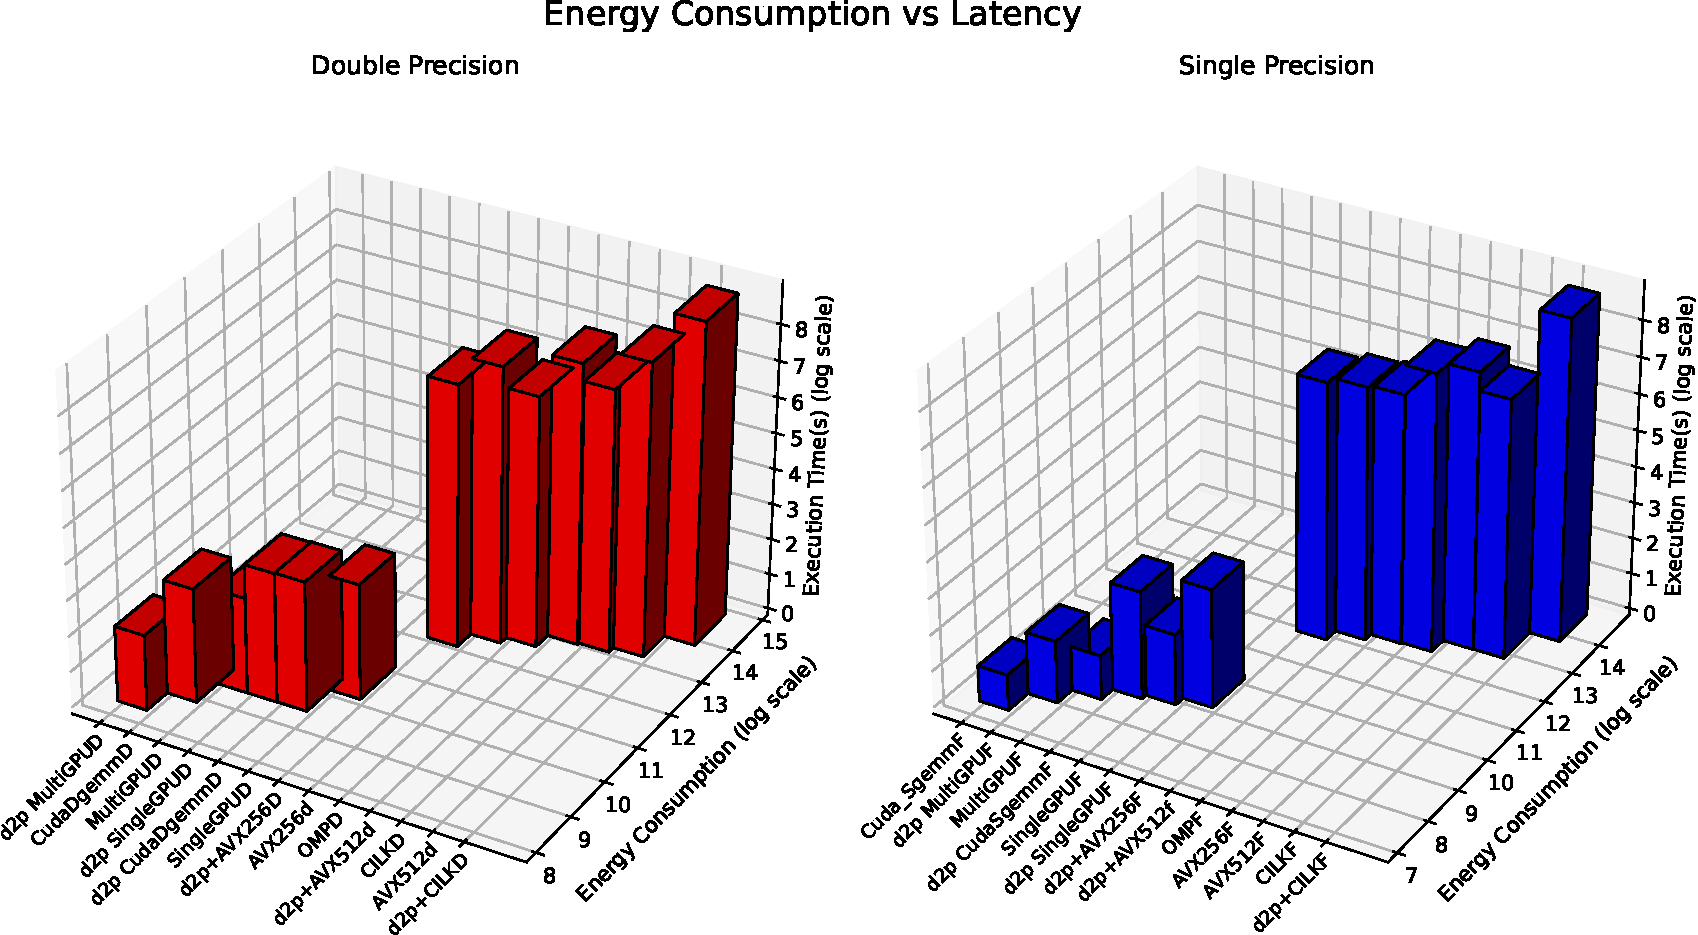
\includegraphics[width=0.9\linewidth]{Images/3d-crop.pdf}
  \vspace{-0.8em}
  \caption{Energy-Execution\_Time-speed\_of\_development plots 
for different implementations with single- and double-precison inputs.}
  \label{fig:3d}
\end{figure*}
\subsection{System Configuration}
We have conducted tests on multiple systems: 
\begin{itemize}
\item Intel(R) Xeon(R) Gold 6240C CPU, 36 physical cores in total in a 2-socket configuration, 2.2MiB L1 cache, 36MiB L2 cache and 49.5MiB L3 cache. Core base frequency is kept at 2.60GHz and the TDP is 150W (Thermal Design Power, which is the average power in watts, that the processor consumes while running at base frequency with all cores active under a complex workload). This system also has two NVIDIA QUADRO RTX 5000 GPUs, each with 16 GB memory and 3,072 CUDA cores, with a maximum power draw of 230W. Evaluated SIMD, CPU-only, Tensorflow-GPU, Tensorflow-CPU, Pytorch-CPU, Pytorch-GPU, BLAS-based, CUDA BLAS based codes on this server. Hybrid parallel codes are also evaluated on this server. 
\item A cluster of two compute nodes and a master node. One of the compute nodes has four A100 cards and the other has two H100 cards. Each with a memory capacity of 80GB. Single GPU and Multigpu codes including using CUDA BLAS libraries are evaluated on these servers. 
\item Jetson Nano has 128 Cuda cores, each with a memory of 4GB and a maximum power draw of 10W.
\item We also employed an AWS Graviton3 processor \texttt{c16\_large}, with 64 cores. This is a cloud-based instance offering VM environment. We have used this to run Arm Neon codes. We have also run experiments on \texttt{c16\_metal}, the baremetal version and observed that the overhead of VM environment is insignificant.
\item Google Colab to test TPU codes in TensorFlow and PyTorch frameworks.
\end{itemize}

During execution, we unrolled the recursion to a depth of 1 to create parallellism for tasks in D2P. This resulted in 8 tasks and we used 4 processes (MPI ranks) to measure the parameters mentioned. 4 processes were considered after we empirically found that the 4-process configuration yielded the best performance (lowest latency). 
We have used perf events for measuring the energy consumption (in Joules) of CPU-based implementations. For measuring GPU energy consumption, we have mainly used Nvidia-smi to monitor GPU power consumption, multiplied it with total execution time to obtain energy consumed by the GPU, and perf to measure the CPU’s overall package energy. Then, we added both energies to calculate the total energy consumed by the GPU and CPU
during the code’s execution.
Our attempt to measure energy consumption on the
the ARM instance on AWS was unsuccessful due to the limited access to performance counters.
\begin{figure*}[htbp]
\centering
\begin{tabular}{cc}
    \begin{minipage}{0.45\linewidth}
        \centering
        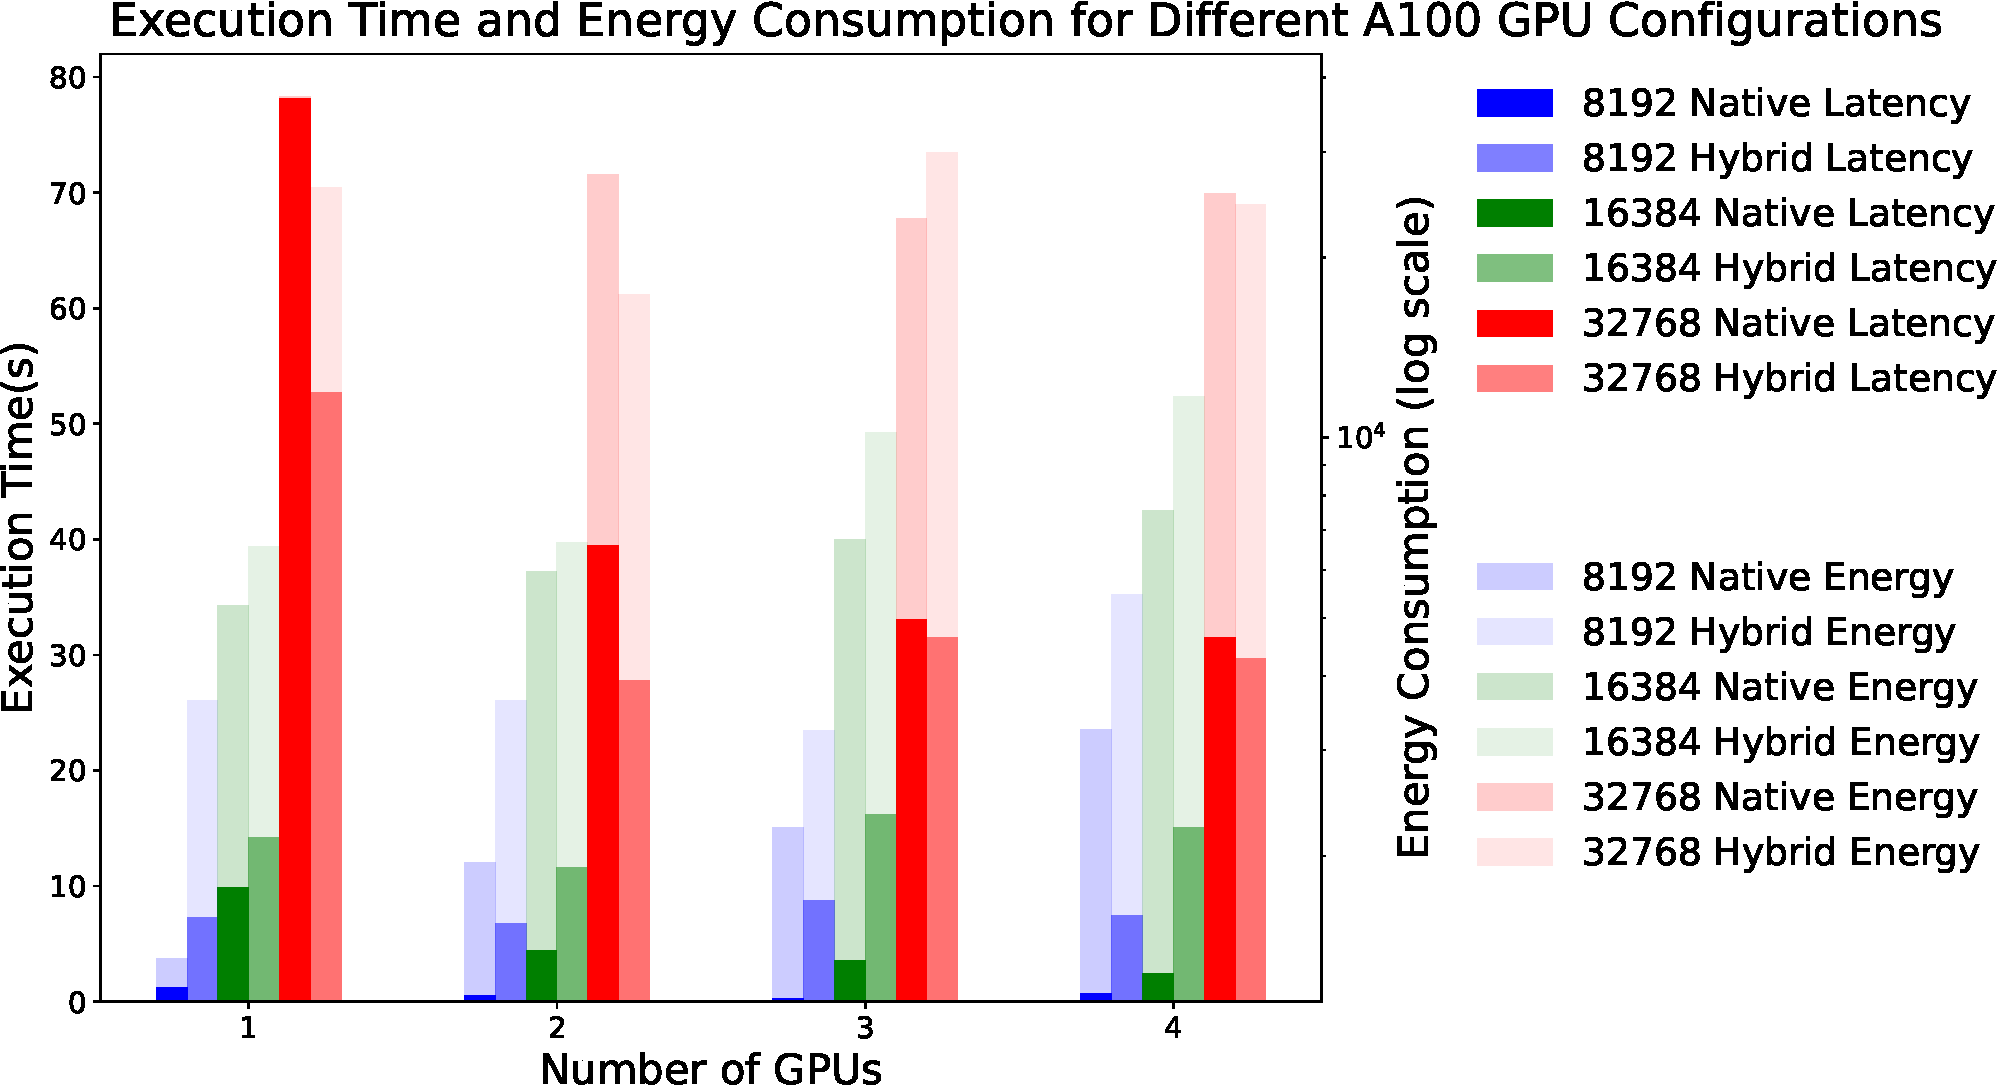
\includegraphics[width=\linewidth, height=5cm]{Images/a100-crop.pdf}
        
    \end{minipage} &
    \begin{minipage}{0.45\linewidth}
        \centering
        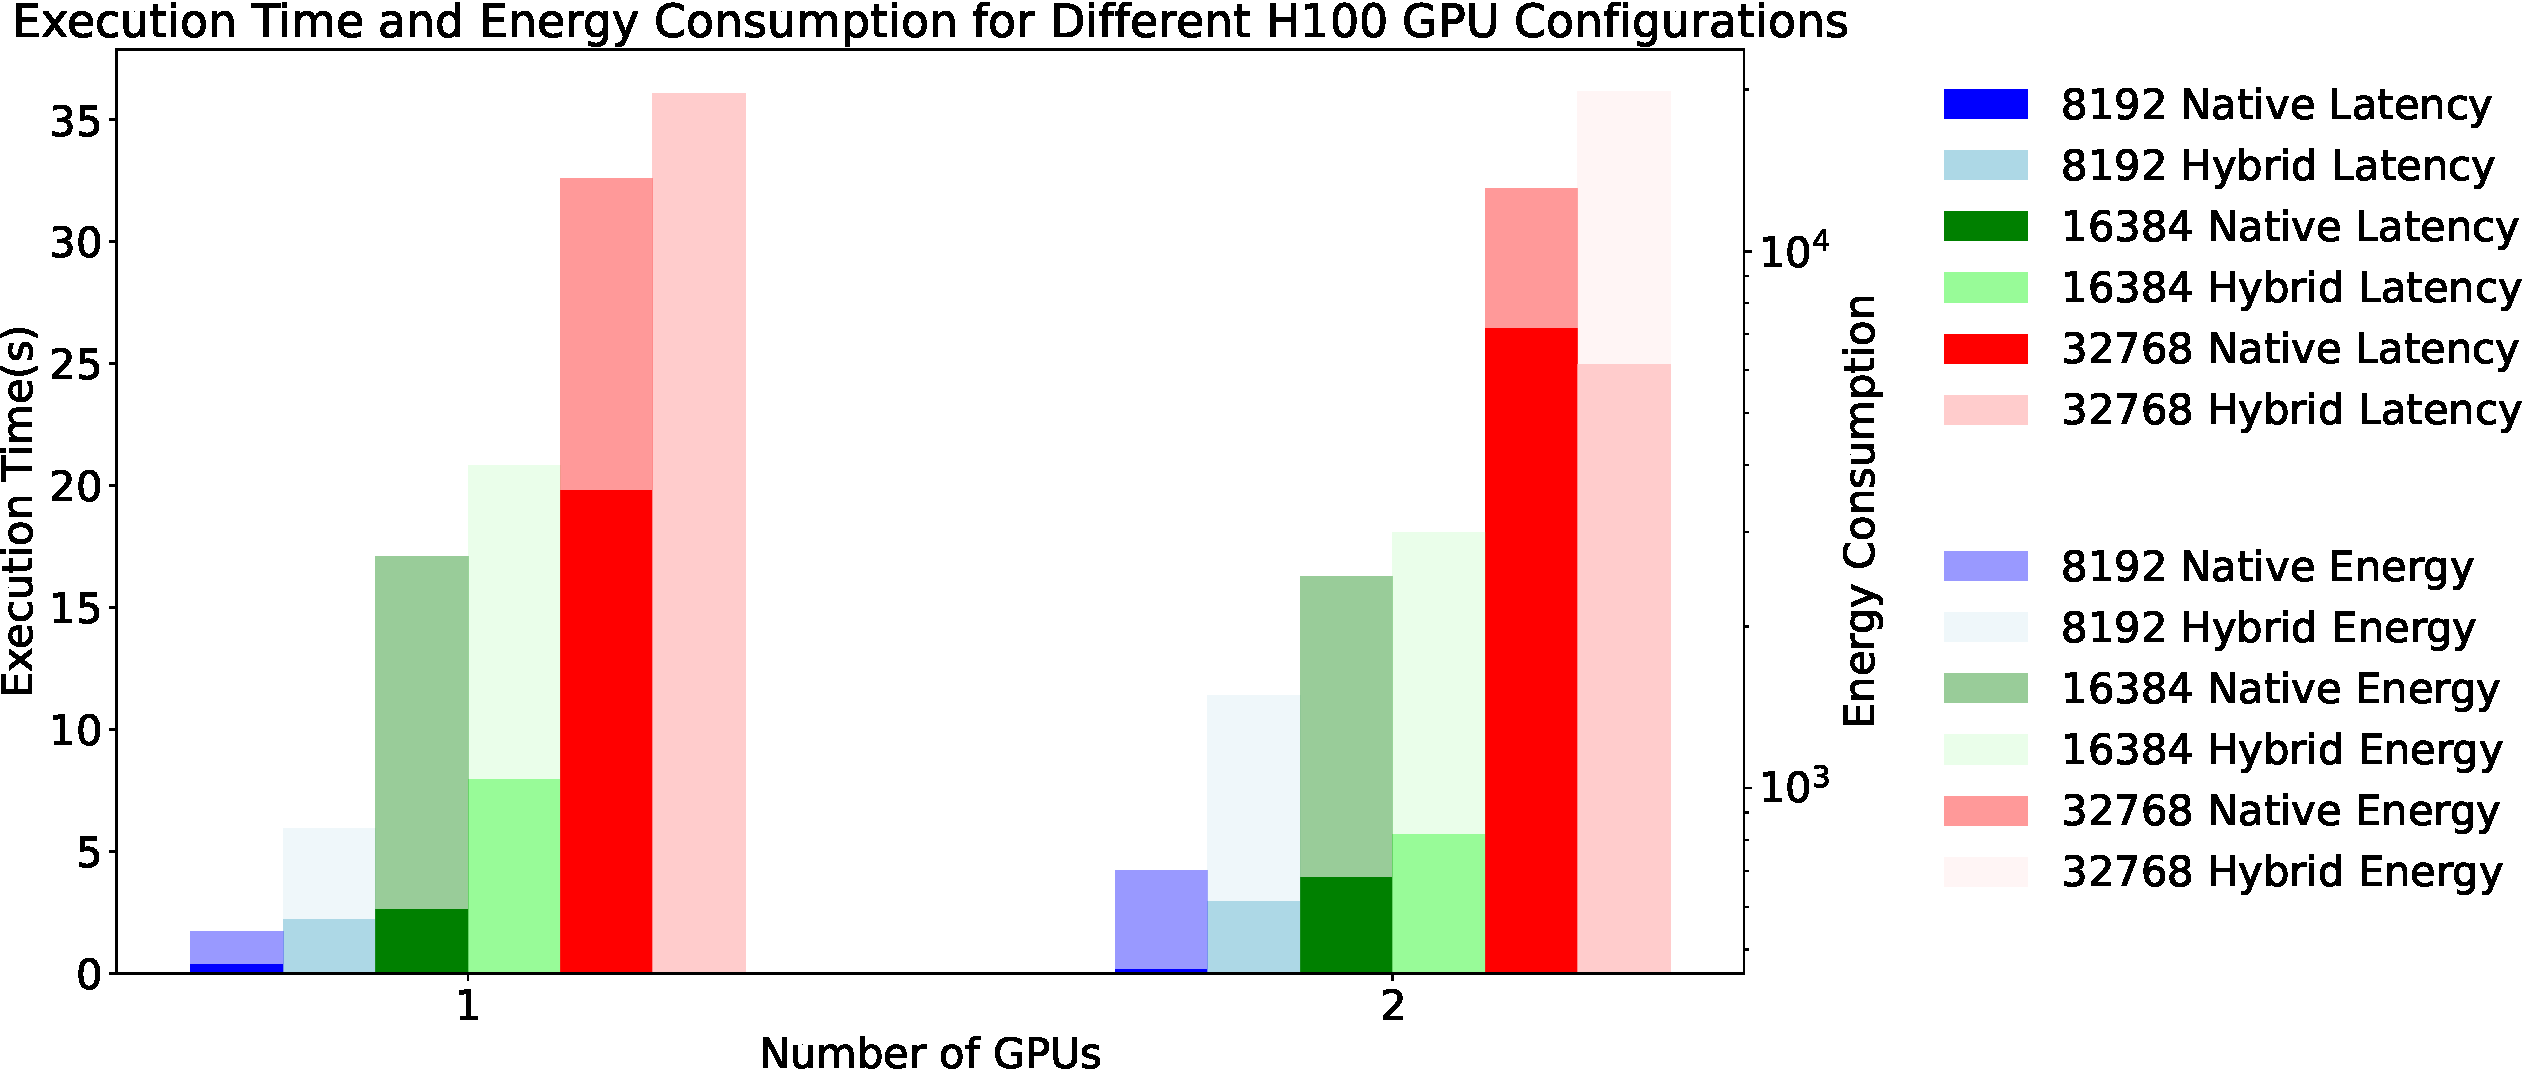
\includegraphics[width=\linewidth, height=5cm]{Images/h100-crop.pdf}
    \end{minipage} \\
\end{tabular}
\caption{Native CUDA-C vs. Augmented CUDA-C comparison on A100 and H100 GPU servers}
\label{fig:A100_H100_nat_vs_aug}
\end{figure*}

\begin{figure*}[htbp]
\centering
\begin{tabular}{cc}
    \begin{minipage}{0.45\linewidth}
        \centering
        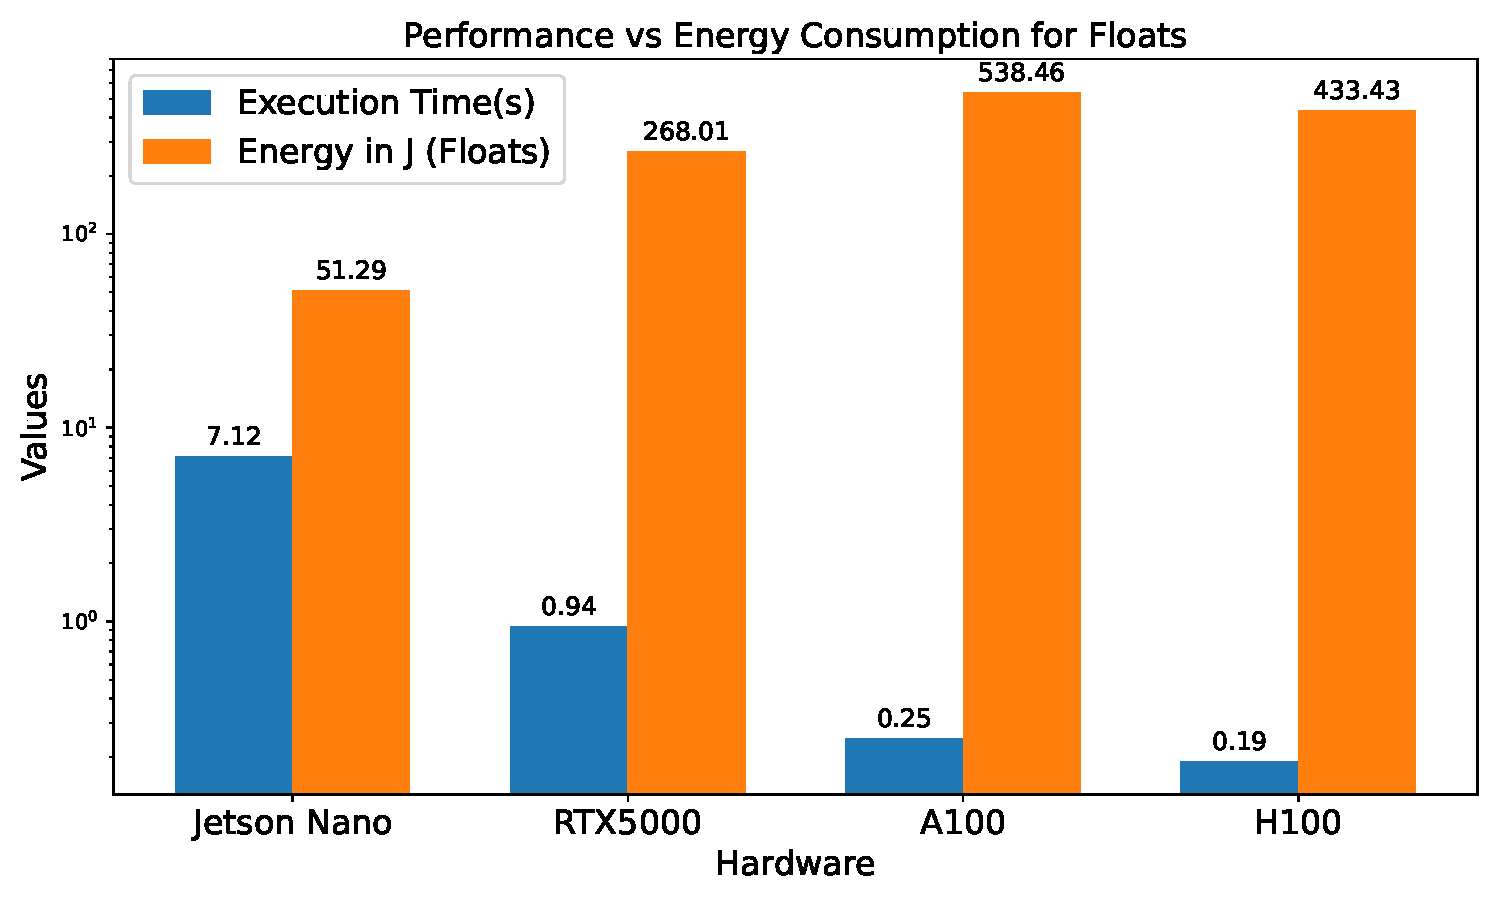
\includegraphics[width=\linewidth]{Images/cuda2.pdf}
    \end{minipage} &
    \begin{minipage}{0.45\linewidth}
        \centering
        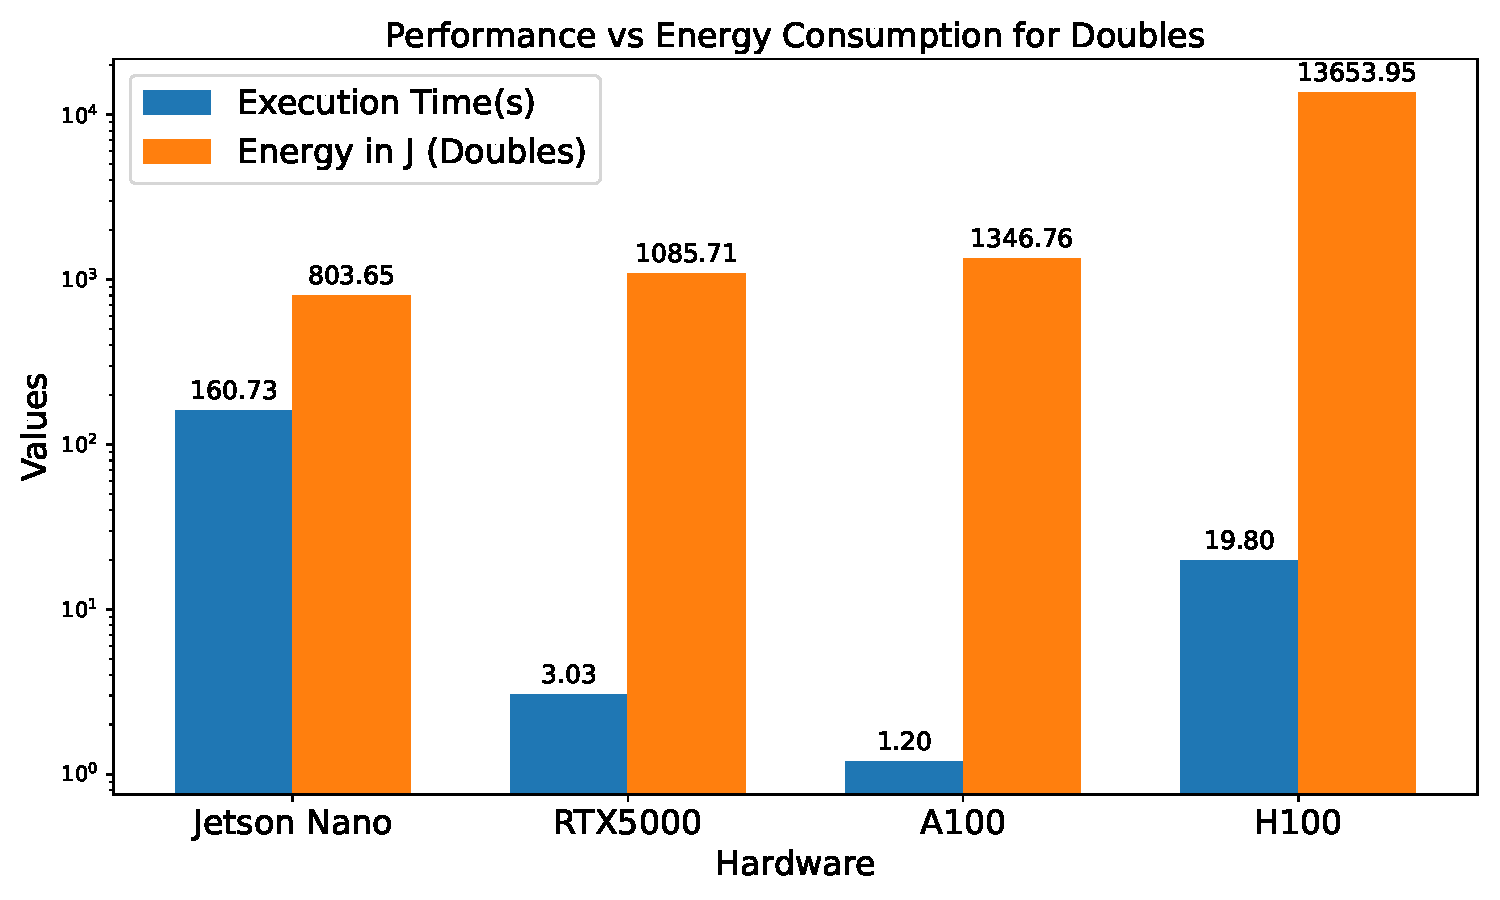
\includegraphics[width=\linewidth]{Images/cuda1.pdf}
    \end{minipage} \\
\end{tabular}
\caption{Performance and Energy consumption of Cuda codes on different Hardwares}
\label{fig:figcudaJNRTX}
\end{figure*}


\subsection{Discussion}

For most codes outside the numerical computing world, double-precision may be an overkill. Even single-precision \texttt{float} data may be over provisioning. In such scenarios, a latency vs. development speed or energy efficiency vs. development speed tradeoff would be more appropriate. Our study shows on multicore execution with \texttt{float} data, OpenMP (OMP) codes deliver almost the same level of performance as that with SIMD codes. In Figure~\ref{fig:3d}, the rhs part shows this result.  OMP codes are much easier to develop and compiler optimizations vectorize the code effectively. Also, we observe that tool-generated hybrid code augmented with AVX performs slightly better than the native code.  If high-precision is necessary, \texttt{double} inputs are to be considered. The lhs part of the Figure shows the results. 

 Figure~\ref{fig:3d} also shows the results with GPU execution. Executions on single and multiple-GPUs, with or without CuBLAS provided APIs, D2P augmented and native are shown. The left half of each part (lhs or rhs) in the figure shows this. We observe that GPU executions consume less energy compared to CPU executions. This is mostly because of the much lesser execution time (latency) on GPUs. It is interesting to note that executions on multiple GPUs consume less energy compared to executions on single GPU. This can be counter-intuitive at first but is due to the overall reduction in execution time  resulting from the distribution of workload on multiple GPUs. Also as expected, increased precision is associated with increased latency and energy consumption. 


In a win-win scenario, we see that tool assisted code implementation yields not only faster development speed but also faster execution. We see that the hybrid parallel code implementation for multi-GPU systems is not only performance portable but executes faster compared to native CUDA code.  Figure~\ref{fig:A100_H100_nat_vs_aug} shows the results.  Also, because of the reduced execution time, hybrid parallel code execution consumes lesser energy. D2P multigpu code was executed with 4 MPI ranks and the base case of the recursion had CUDA-kernel to distribute the workload across available GPU cards on the system. The native code was a plain CUDA code and had kernel to distribute the workload across available GPU cards. The executions were performed with varying number of GPU cards on RTX5000, A100, and H100 systems (Figure~\ref{fig:1} shows the results with RTX5000 card). We see that the hybrid parallel code outperformed native code on these systems for double precision numbers by achieving higher total memory throughput while having slightly lower compute throughput. There was no significant performance impact from this slight variation in compute throughput. Whereas for single  precision values, the native code outperformed the hybrid code in terms of memory and computation throughput. As a result, a similar behaviour as doubles is not seen in floats. Another interesting observation is that the difference in the latency between the cudaSgemm and CudasingleGPU implementations vanishes from 4k to 8k.To understand this behaviour, we profiled the codes using profilers mentioned in previous section. Through the profiled information, we found that the computational intensity of both codes almost doubles from 4k to 8k to 16k, and for 16k-sized matrices, we see that cudaSgemm executes faster than cudasingleGPU. From this, we infer that the Cuda library-based approach is beneficial for matrix sizes greater than or equal to 8k. We continue the discussion on GPU executions with a focus on energy consumption next.
%\begin{figure*}[h]
%   \centering
%   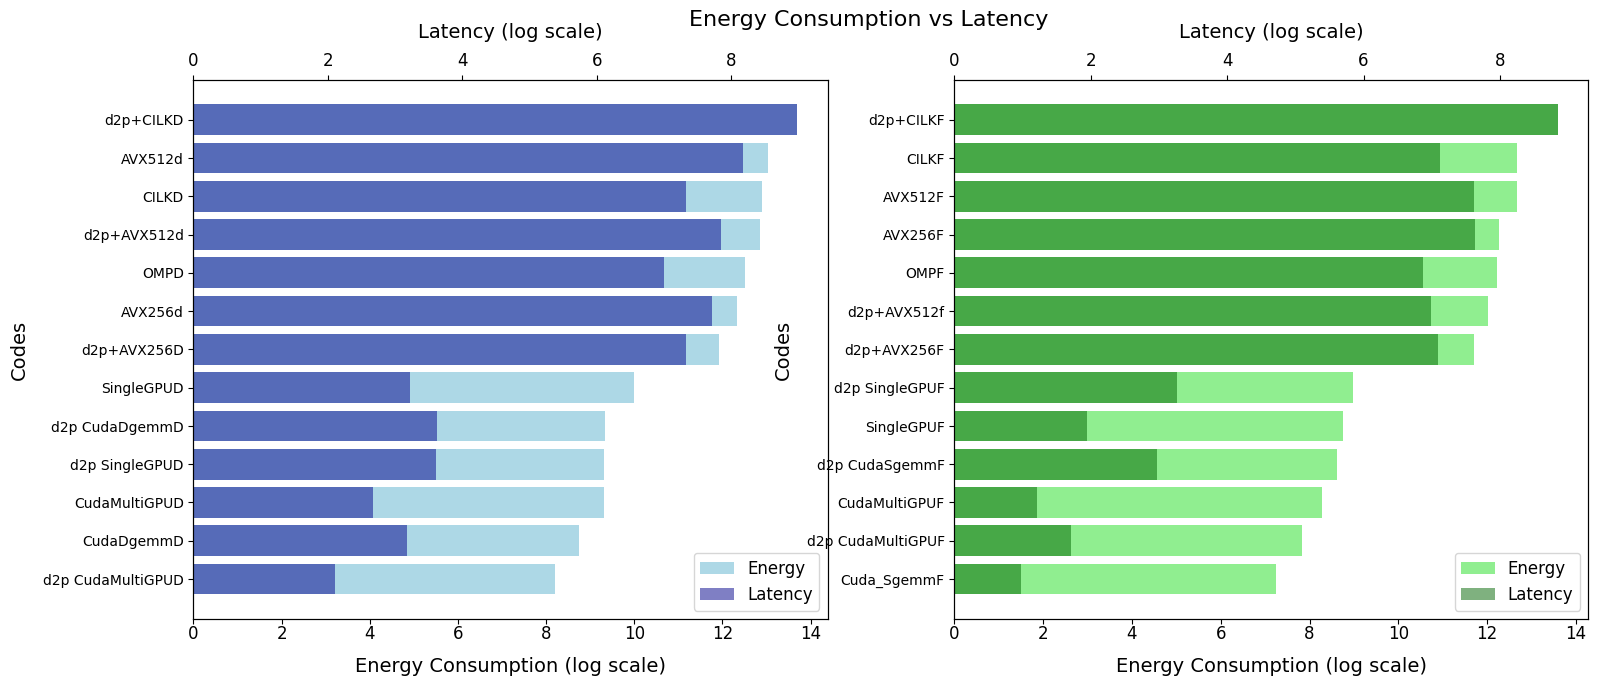
\includegraphics[width=0.8\textwidth]{2d dodgeplot1.png}
%    \caption{Consolidated Plot for easy analysis}
%    \label{fig:dodge}
%\end{figure*}



% For displaying results of next section on the same page
\begin{figure*}[ht]
\centering
\begin{tabular}{ccc}
    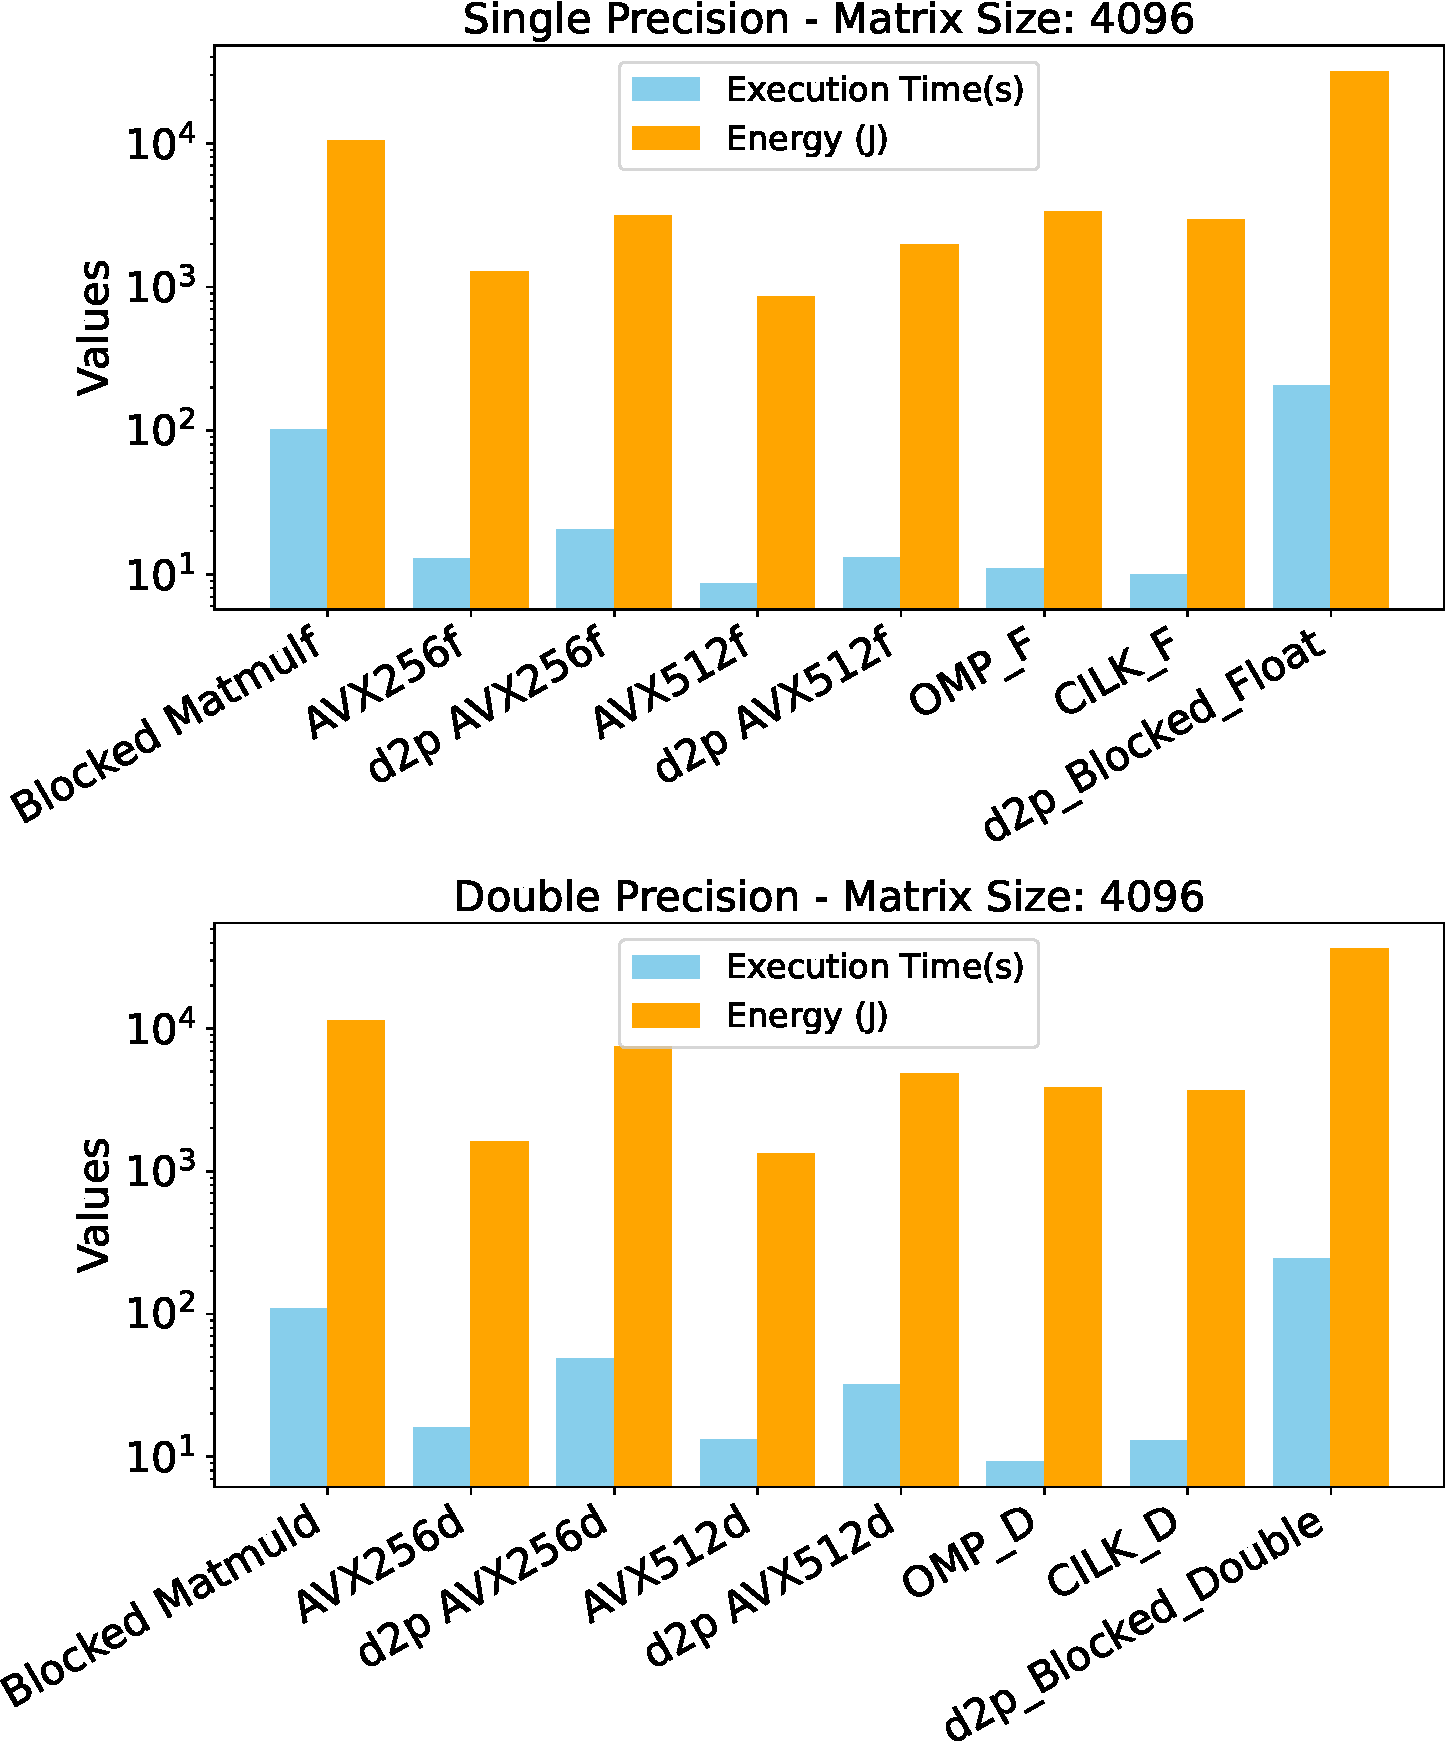
\includegraphics[width=0.32\linewidth,height=7cm]{Images/cpu4k-crop.pdf} &
    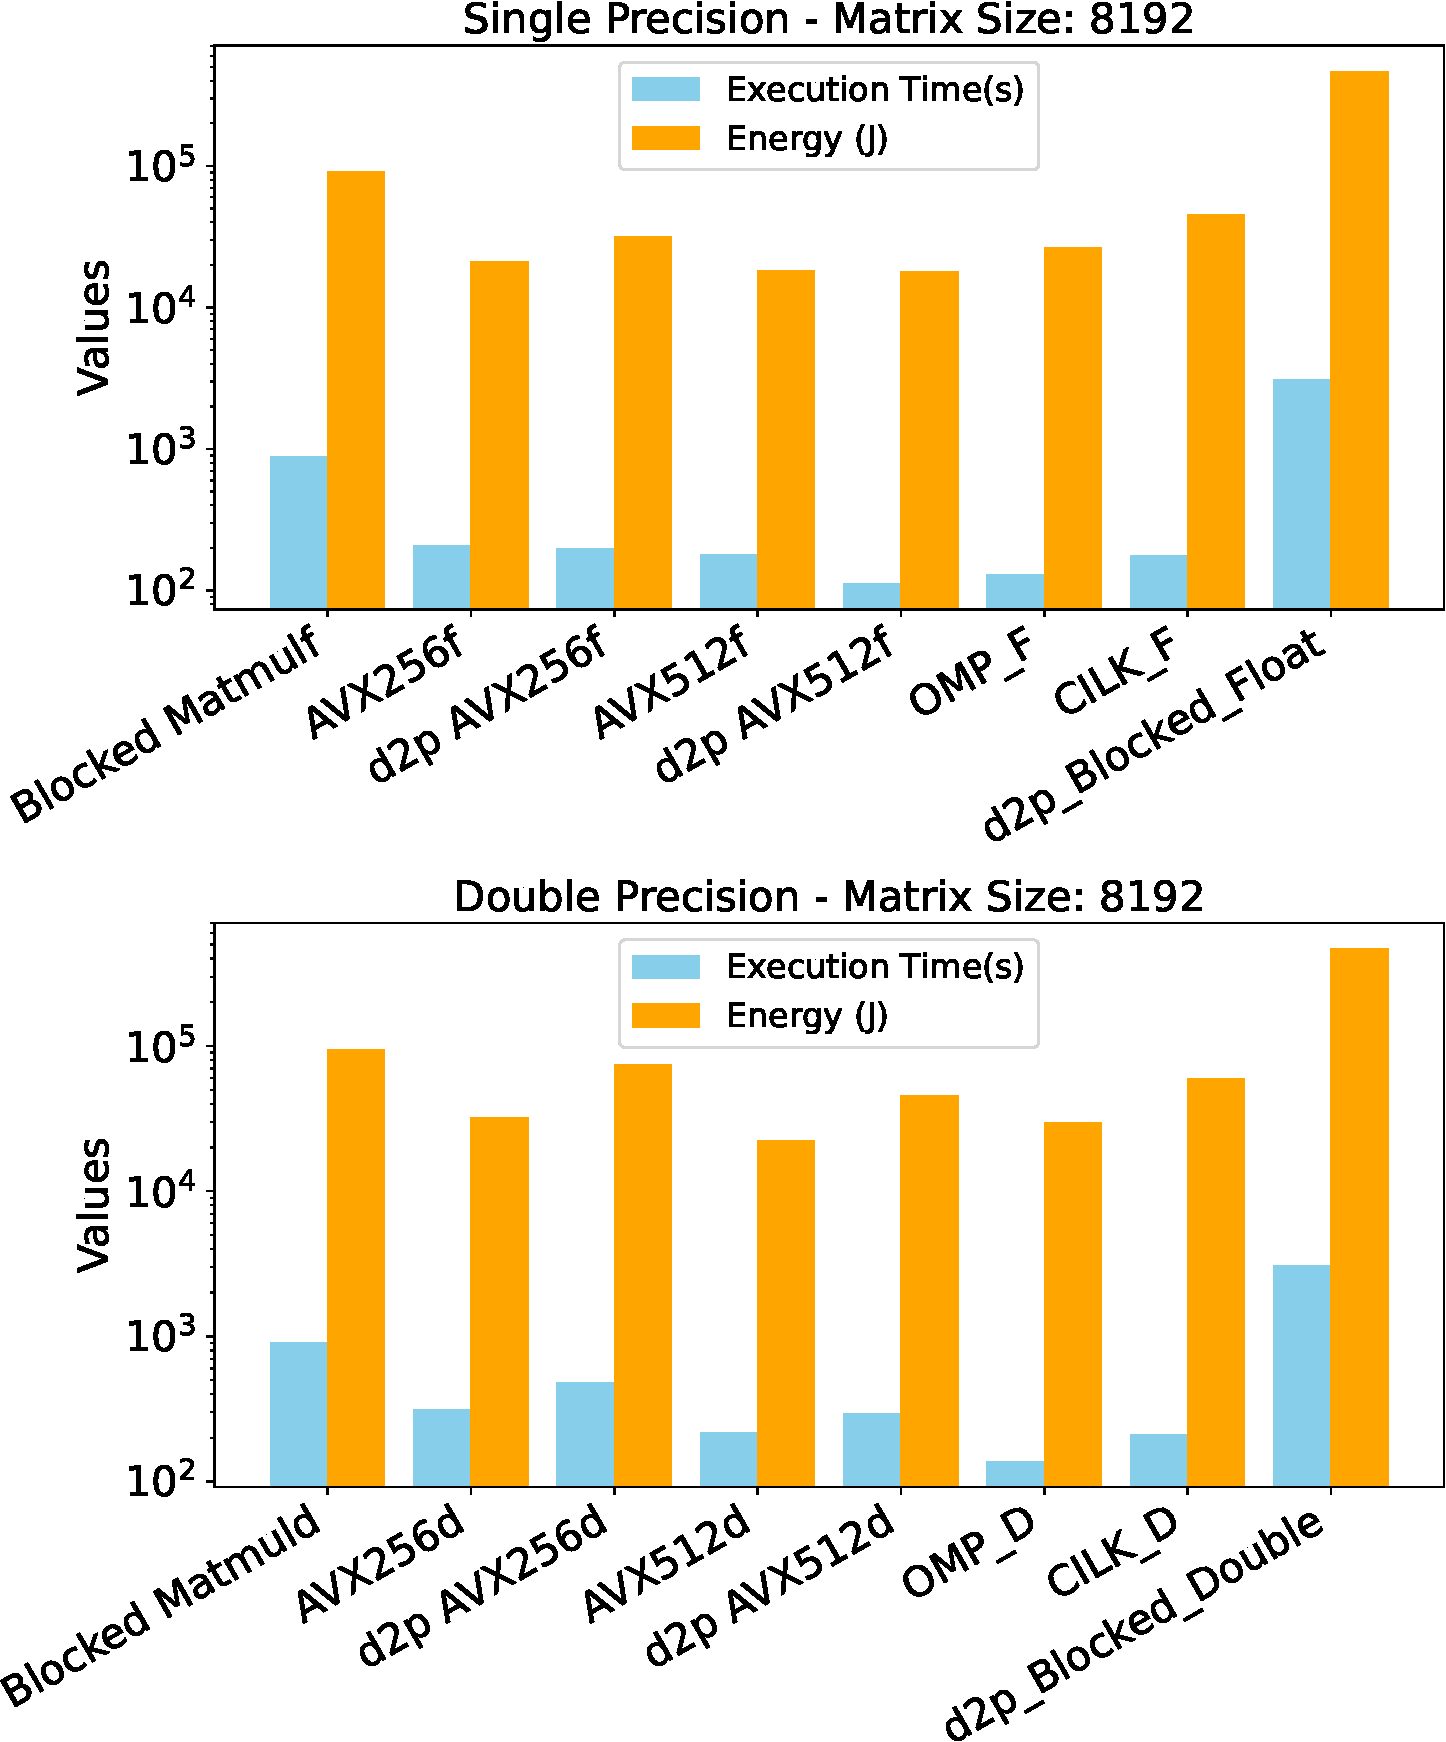
\includegraphics[width=0.32\linewidth,height=7cm]{Images/cpu8k-crop.pdf} &
    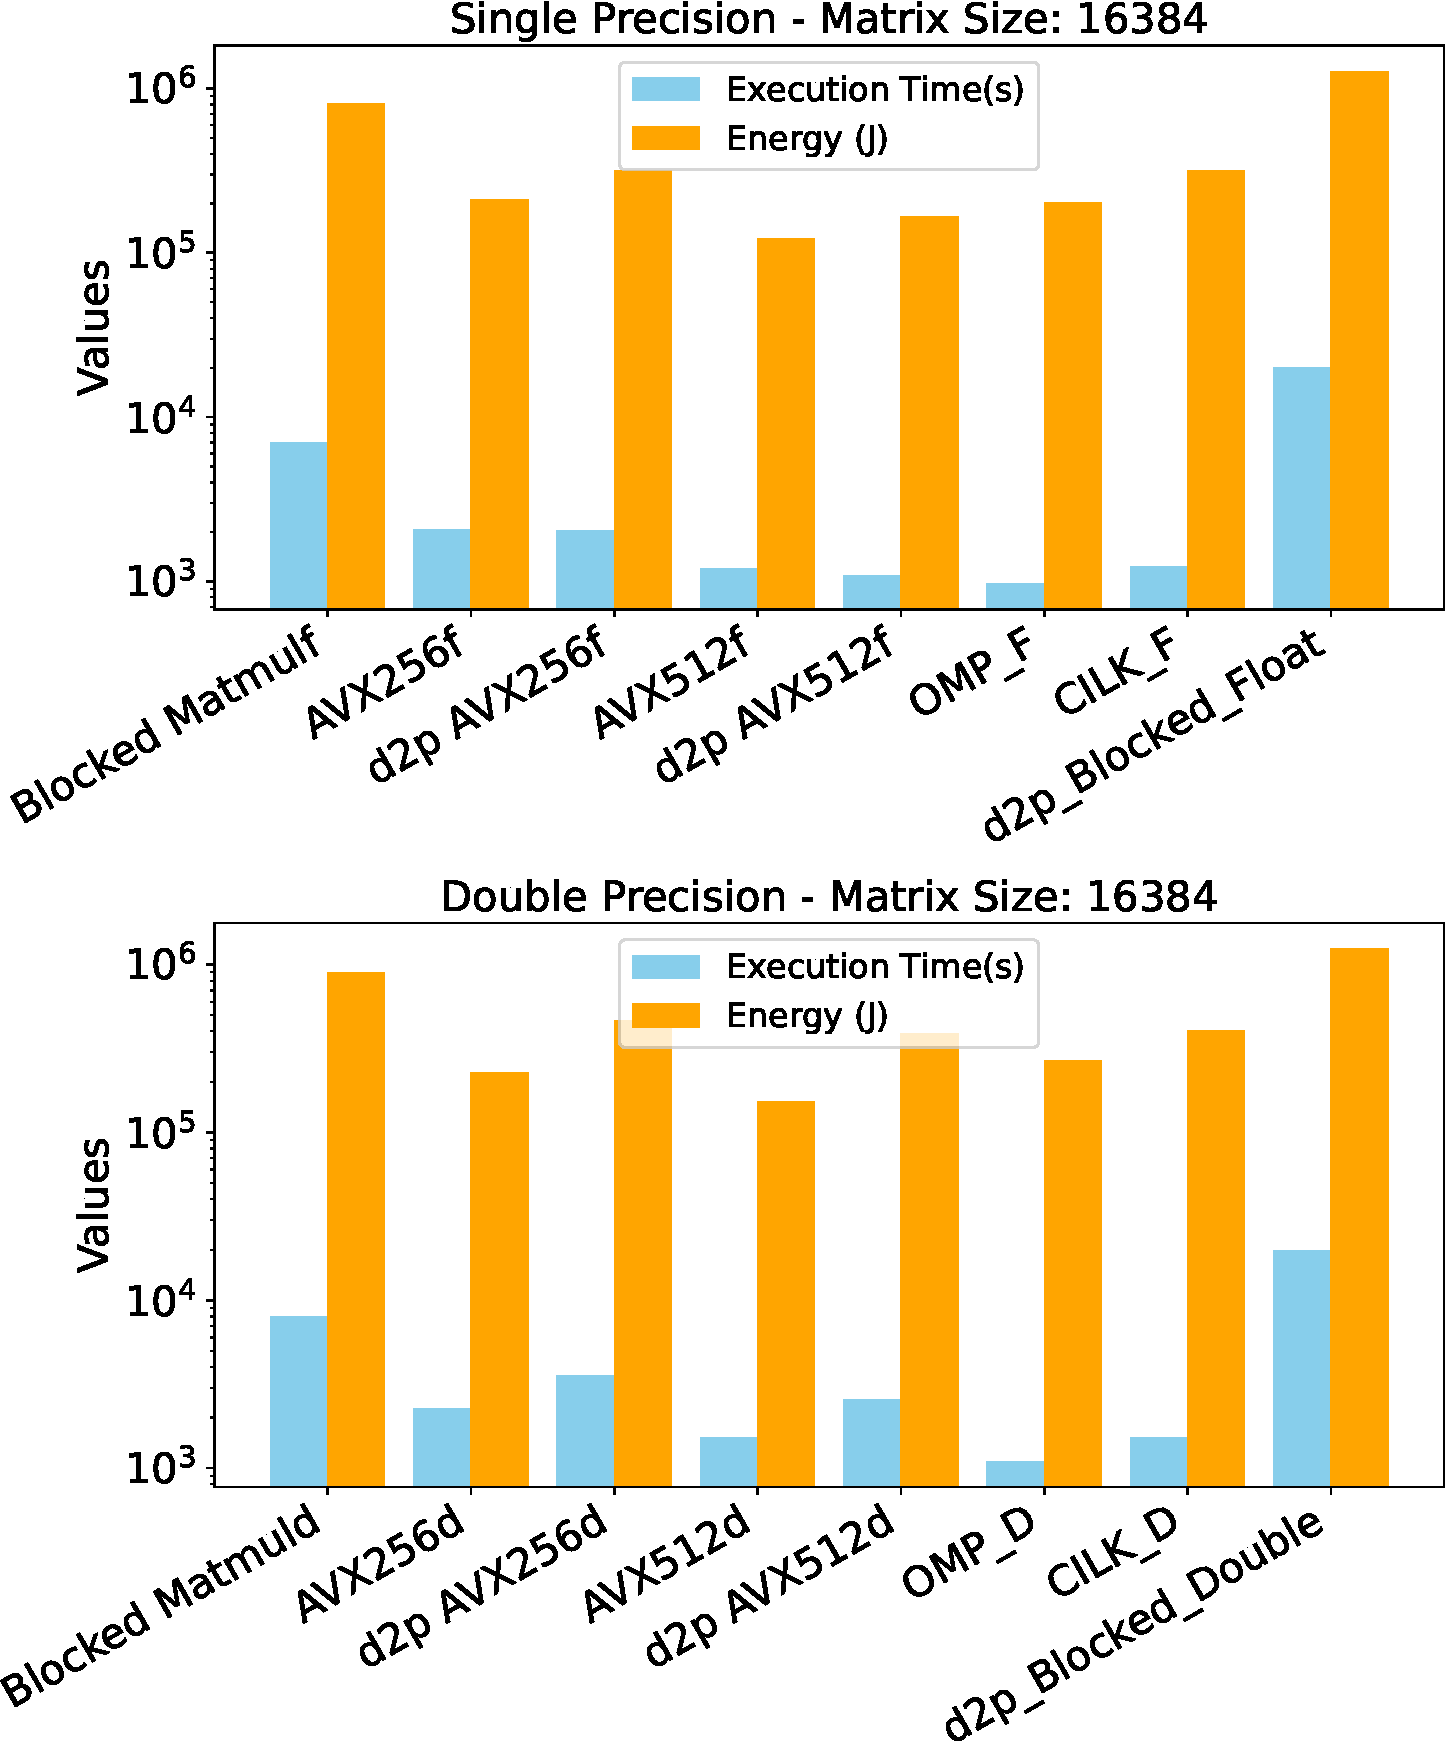
\includegraphics[width=0.32\linewidth,height=7cm]{Images/cpu16k-crop.pdf}\\ 
    (a) 4k & (b) 8k & (c) 16k \\
\end{tabular}
\caption{Performance characteristics on CPU cores for sizes 4k to 16k}
\label{fig:cpumulticore}
\end{figure*}




\begin{comment}
\begin{figure}[h!]
  \centering
  \includegraphics[width=1.0\linewidth]{A100.png}
  %\vspace{-0.8em}
  \caption{Native CUDA-C vs. Augmented CUDA-C comparison on A100 with matrix sizes scaling from 8k to 32k.}
  \label{fig:A100}
\end{figure}
\end{comment}



%\subsection{Experimental Analysis}
\paragraph{Energy consumption on GPUs and Jetson Nano} 
Figure~\ref{fig:figcudaJNRTX} shows the energy consumption when we execute native matrix-multiplication code with 8k input matrix size. We use a single GPU card on each of the GPU-servers in these experiments. The figure shows the data for both single- and double-precision inputs. With single-precision input data, Jetson Nano execution is 37$\times$ slower than the most powerful H100 GPU execution. In contrast, the Jetson Nano is energy efficient compared to H100 by 8.5$\times$. With double precision input data,  Jetson Nano code is slower by 48.7$\times$ compared to RTX100, 133$\times$ compared to A100, and only 8.4$\times$ compared to H100. We observe that H100 performance falls below that of A100 for double-precision data and are doing further study to understand the reason. Energy consumption-wise, Jetson Nano is 1.7$\times$ more efficient compared to the best performing A100 GPU for double-precision inputs. Beyond 8k input matrix sizes, we start seeing overflow in Jetson Nano. This experiment shows that in a scenario with lower precision requirement and no strict latency requirement, Jetson Nano can be very energy efficient when single-precision \texttt{float} data is chosen.    

%\input{Figures/Colab TPU results using TensorFlow and PyTorch}
\begin{figure*}[h]
    \centering
    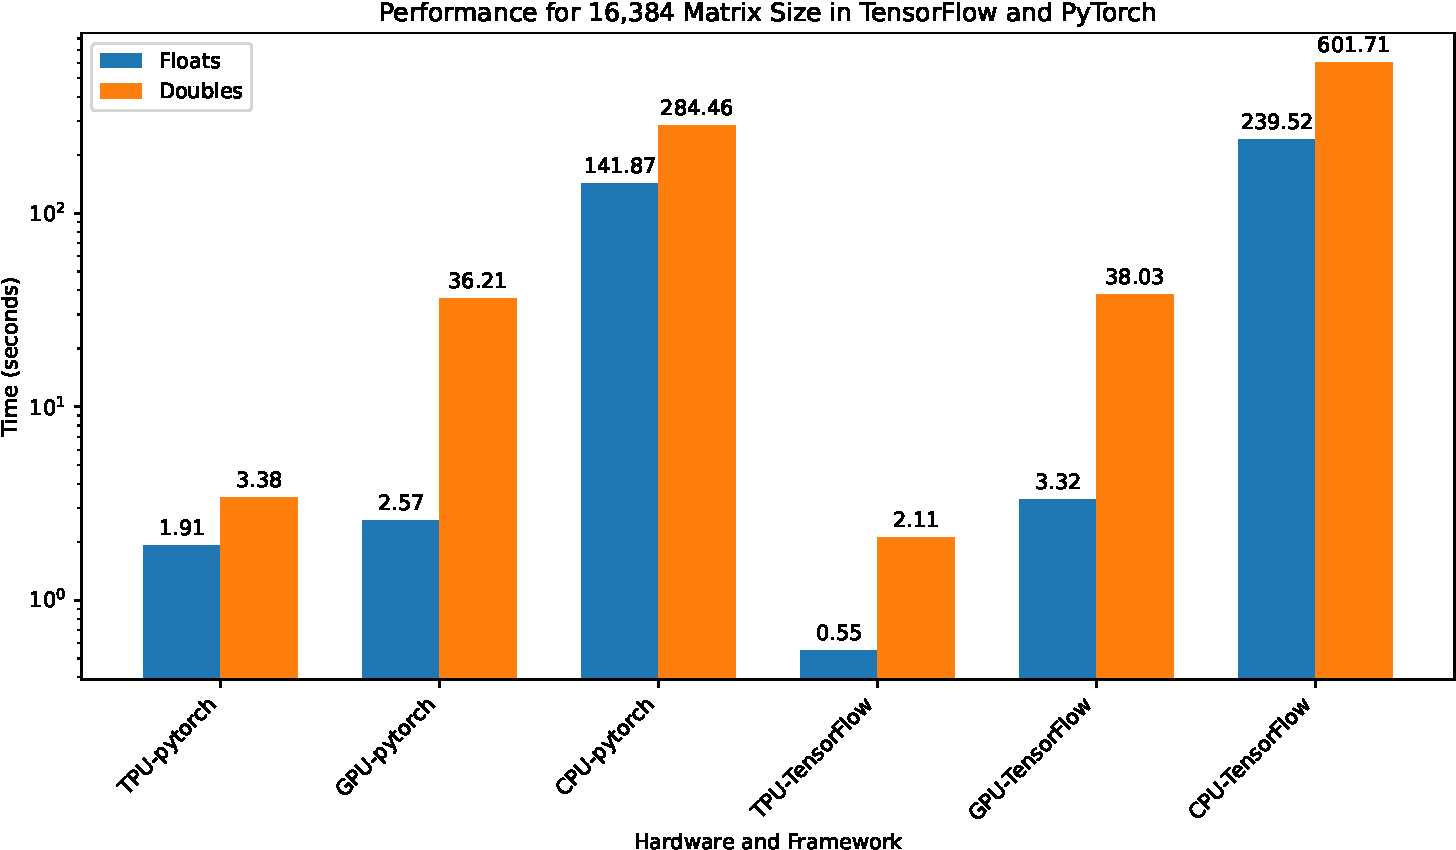
\includegraphics[width=0.75\textwidth]{Images/TF&Py-crop.pdf}
    \caption{Colab TPU results using TensorFlow and PyTorch}
    \label{fig:TPU}
\end{figure*}
\paragraph{TPU executions}
We explored TPU performance using TensorFlow and PyTorch for matrix multiplication on Google Colab, comparing it to GPU v4 and CPU for matrix sizes varying from 4k to 16k as before. Due to restricted hardware access, power consumption details were not available. For a 16k matrix, PyTorch showed that the TPU was 74x faster than the CPU and 1.2x faster than the GPU for single precision, and 84x faster than the CPU and 10x faster than the GPU for double precision. TensorFlow results indicated that the TPU was 6x faster than the GPU and 435x faster than the CPU for single precision, and 280x faster than the CPU and 18x faster than the GPU for double precision. The findings focus on  the trade-offs among latency and energy consumption in multi-GPU setups and the performance of TPUs for  matrix operations. Figure~\ref{fig:TPU} shows the results.

\paragraph{multicore execution on x86 and Arm}
We begin with multicore execution on x86 architectures. We have evaluated blocked (tiled), OMP, Cilk, AVX, AVX2, D2P with (tiled, AVX, and AVX2) variants on the RTX5000 system (we have named this system as RTX5000 but not used the GPU card in these experiments.). Figure~\ref{fig:cpumulticore} shows the details. 

As we increase the matrix size from 4k to 16k, the better-performing and energy-efficient programming model shifts. In the case of single precision, AVX512f is energy-efficient at 4k, whereas the OMP and D2P integrated with AVX512 become faster at 16k. On the other hand, for double precision, the OMP code constantly has lower latency, whereas  AVX512d remains energy-efficient across all matrix sizes. Figure~\ref{fig:armvsx86} shows the results of executing on Arm based instance on AWS. Figure~\ref{fig:arm} shows the trend observed on ARM systems, i.e., Native NEON code performs better than Hybrid NEON code for all the matrix sizes for single and extended precision.In figure \ref{fig:armvsx86}, observe that OMP and CILK codes on ARM perform better than x86.

We have also explored library-based methods like CBLAS and MKL implementations, where MKL outperformed with significantly better execution time and lower energy consumption than CBLAS.  We also implemented the hybrid implementations, d2p\_cblas and d2p\_MKL, which showed improved performance and energy consumption relative to CBLAS. However, they still are less efficient than MKL. The AVX-based implementations combined with Cilk or OpenMP, exhibited the highest execution times and energy consumption among all methods.  The table~\ref{tab:comparison} displays the detailed analysis for each implementation. Apart from the above methods, we have also leveraged Kokkos framework to explore performance portability aspect. We observed that KOKKOS introduces an abstraction overhead, which results in it being 2.3x slower than native CPU and 15x slower than native CUDA codes, it is discussed in detail in the \cite{kokkos}.

\begin{table}[htbp]
    %\centering
    $$
    \setlength{\tabcolsep}{2pt}
    \begin{tabular}{|c|c|c|}
        \hline
        \textbf{Codes} & \textbf{Execution Time (s)} & \textbf{Energy Consumed (J)} \\
        \hline
        CBLAS\_D      & 15.83   & 4753.77  \\
        MKL\_D        & 9.15    & 2452.98  \\
        d2p\_cblasD   & 14.82   & 3940.68  \\
        d2p\_MKLD     & 14.95   & 3953.05  \\
        AVX+ CILKD    & 39.83   & 12037.66 \\
        AVX+ OPENMPD  & 40.31   & 11156.25 \\
        \hline
    \end{tabular}
    $$
    \caption{Comparison of execution time and energy consumption across different implementations for 16k-sized matrices.}
    \label{tab:comparison}
\end{table}


Table~\ref{tab:co} displays the cost of ownership details.Traditionally, the cost of ownership is computed in dollars.In our study, we adopted a metric that is generally used in the semi-conductor industry : picoJoules per bit. Aiming to provide an estimation of the amount of energy spent per bit of computation. This metric provides a standardised approach that takes into account the various geographical representations and cost structures. Using this metric provides a common representation that is universally applicable for a comparison of energy efficiency across diverse regions. 
The data in Table~\ref{tab:co} shows that harnessing accelerators like the Jetson Nano and exploiting the benefits of multi-GPU setups offer higher energy efficiency. In contrast, other implementations like AVX-Native, CILK, and OMP have high energy consumption. Optimized implementations like D2p AVX substantially reduce energy usage.


%TODO:More explanation about Total cost of Ownership

\begin{figure}[htbp]
  \centering
  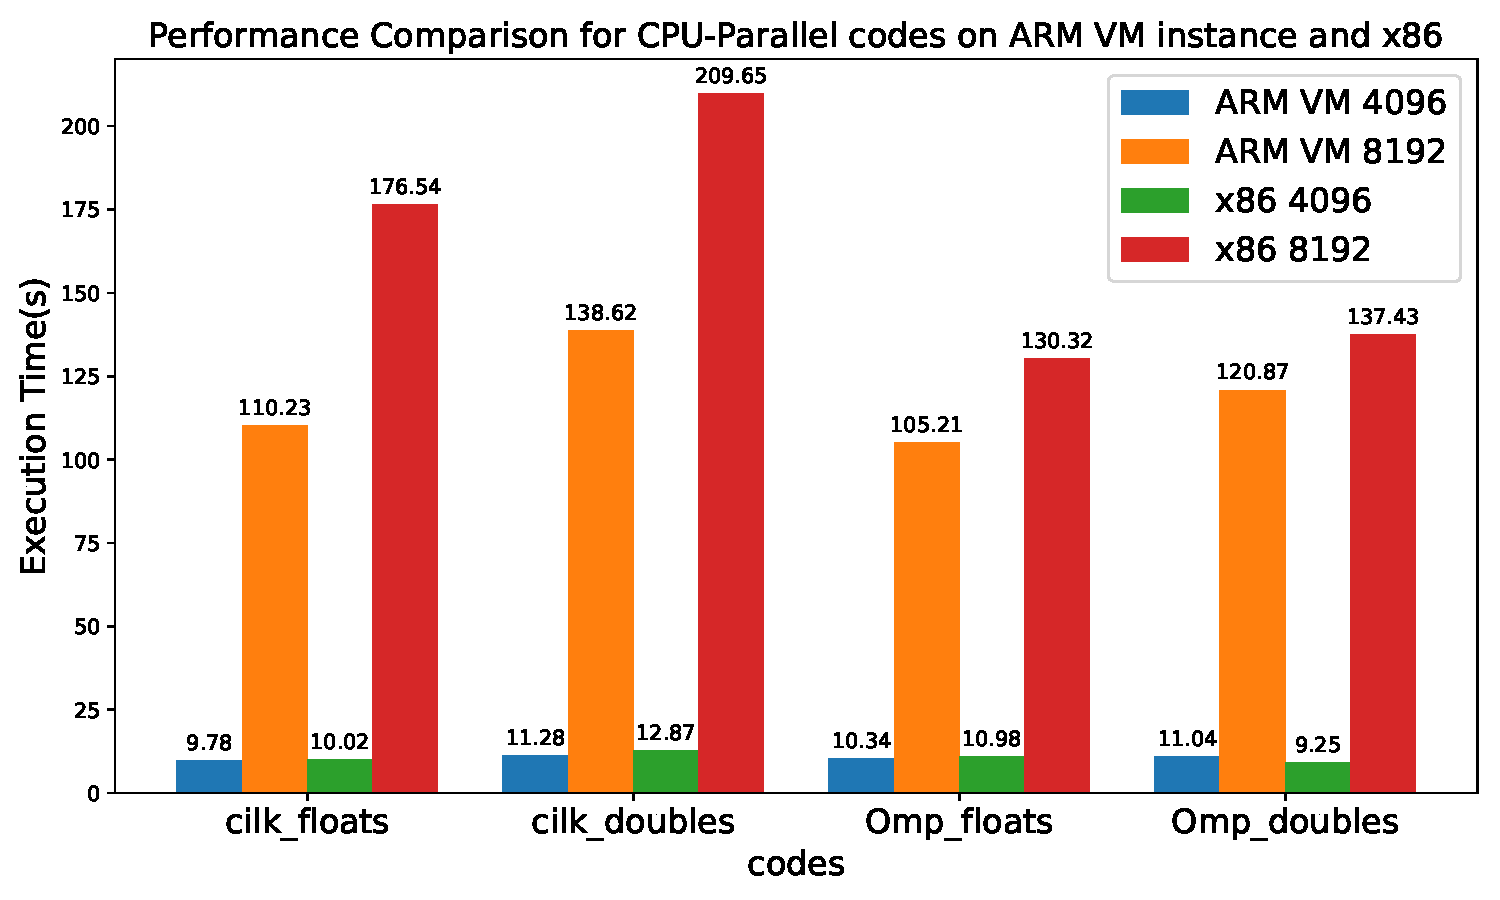
\includegraphics[width=1.0\linewidth]{Images/ARMvsx86.pdf}
  %\vspace{-0.8em}
  \caption{Performance of CPU Parallel codes on ARM vs x86.}
  \label{fig:armvsx86}
\end{figure}
%\begin{figure*}[ht]
\centering
\caption{Comparison of Single and Double Precision GPU Codes on RTX5000 and Jetson Nano}

\begin{subfigure}{0.45\linewidth}
    \centering
    \includegraphics[width=\linewidth]{Images/newRTXJNF.png}
    \caption{Single Precision 4k}
    \label{fig:RTXJNfloat4k}
\end{subfigure}
\hfill
\begin{subfigure}{0.45\linewidth}
    \centering
    \includegraphics[width=\linewidth]{Images/newRTXJNF8k.png}
    \caption{Single Precision 8k}
    \label{fig:RTXJNfloat8k}
\end{subfigure}

\begin{subfigure}{0.45\linewidth}
    \centering
    \includegraphics[width=\linewidth]{Images/newRTXJND.png}
    \caption{Double Precision 4k}
    \label{fig:RTXJNdouble4k}
\end{subfigure}
\hfill
\begin{subfigure}{0.45\linewidth}
    \centering
    \includegraphics[width=\linewidth]{Images/newRTXJND8k.png}
    \caption{Double Precision 8k}
    \label{fig:RTXJNdouble8k}
\end{subfigure}
\label{fig:gpu}
\end{figure*}

\input{Figures/Native Vs Hybrid using NEON intrinsics}

%\input{Figures/Latency-Energy Consumption trade-off for Multi-GPU on NVIDIA A100 & H100 GPUs}


\begin{figure*}[htbp]
\centering
\caption{Native Vs Hybrid using NEON intrinsics}
\begin{subfigure}{0.45\linewidth}
    \centering
    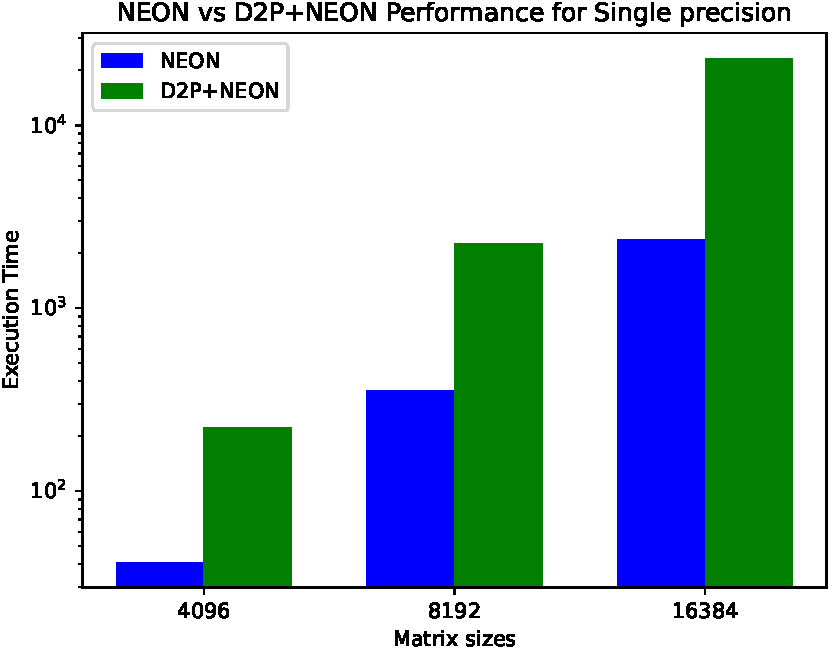
\includegraphics[width=0.90\linewidth]{Images/d2pvsNEONf-crop.pdf}
    \caption{Single precision}
    \label{fig:arm_float}
\end{subfigure}
\hfill
\begin{subfigure}{0.45\linewidth}
    \centering
    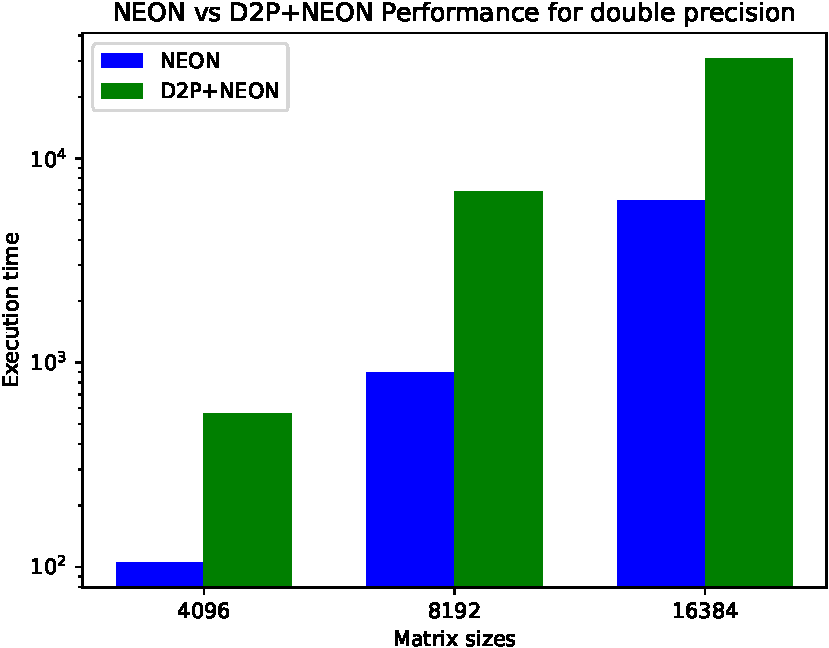
\includegraphics[width=0.90\linewidth]{Images/d2pvsNEONd-crop.pdf}
    \caption{Double precision}
    \label{fig:arm_double}
\end{subfigure}
\label{fig:arm}
\end{figure*}  


The performance peak percentages across the different hardware architectures display apparent differences in their ability to maximise efficiency as shown in Table \ref{tab:ppp}. The A100 demonstrates strong scalability in hybrid code, especially with multiple GPUs, reaching a peak of 24.47\% and outperforming its native counterpart. On the other hand, H100  performs well for native single-GPU execution, achieving 36.64\%, but it reduces for multiple gpus, indicating less scalability in multi-GPU setups. In contrast, the Quadro RTX 5000 performs poorly in single-GPU execution (3.14\%) but benefits significantly from hybrid parallelism in multi-GPU configurations, achieving 9.07\% peak performance. A common takeaway from these results is that hybrid parallelism yields better performance in multi-GPU setups, as seen with all the hardware, while single-GPU performance is maximised in native execution, especially with the H100.

As our future work, we will extend our experimentation on clusters with GPU nodes and power measurements on Arm based systems and TPUs.
\begin{table}[htbp]
$$
\begin{array}{|l|l|}
\hline \text {\textbf{Versions}} & \textbf{ picoJoules/bit } \\
\hline \text { D2p AVX } & 1019.98 \\
\hline \text { D2p cuda } & 69.51 \\
\hline \text { D2p Sgemm } & 66.88 \\
\hline \text { D2p multigpu } & 40.03 \\
\hline \text { OMP } & 1501.29 \\
\hline \text { CILK } & 2587.76 \\
\hline \text { Jetson Nano} & 2.91 \\
\hline \text { AVX-Native} & 6915.32 \\
\hline
\end{array}
\vspace{-0.25cm}
$$
\caption{Cost of ownership}
\label{tab:co}
\end{table}


\begin{table}[htbp]
\centering
\begin{tabular}{|c|c|c|c|}
\hline
\textbf{Hardware} & \textbf{GPUs} & \textbf{Native (\%)} & \textbf{Hybrid (\%)} \\ \hline
A100              & 1             & 9.29                 & 13.76                \\ \hline
A100              & 2             & 18.37                & 26.14                \\ \hline
A100              & 3             & 21.97                & 23.04                \\ \hline
A100              & 4             & 23.06                & 24.47                \\ \hline
H100              & 1             & 36.64                & 20.11                \\ \hline
H100              & 2             & 8.87                 & 9.40                 \\ \hline
Quadro RTX        & 1             & 3.136                & 2.125                \\ \hline
Quadro RTX        & 2             & 5.822                & 9.069                \\ \hline
\end{tabular}
\caption{Peak Performance Percentages for Native and Hybrid Codes on Different Hardware}
\label{tab:ppp}
\end{table}





